% ============================================================================
% Descubrimiento Evolutivo de Estrategias Cuantitativas en Criptomonedas
% Universidad del CEMA
% ============================================================================
\documentclass[12pt,a4paper]{article}

% --- Idioma ---
\usepackage[spanish,es-tabla,es-noquoting]{babel}
\usepackage[utf8]{inputenc}
\usepackage[T1]{fontenc}

% --- Matemáticas ---
\usepackage{amsmath,amssymb,amsthm}

% --- Gráficos y tablas ---
\usepackage{graphicx}
\usepackage{booktabs}
\usepackage{multirow}
\usepackage{float}

% --- Código y algoritmos ---
\usepackage{listings}
\usepackage[ruled,vlined,linesnumbered]{algorithm2e}
\SetAlgorithmName{Algoritmo}{Algoritmo}{Lista de Algoritmos}

% --- Referencias y enlaces ---
%\usepackage[numbers,sort&compress]{natbib}
\usepackage[colorlinks=true,linkcolor=blue!60!black,citecolor=green!50!black,urlcolor=blue!70!black]{hyperref}

% --- Layout ---
\usepackage[margin=2.5cm]{geometry}
\usepackage{setspace}
\onehalfspacing
\usepackage{parskip}

% --- Colores para listings ---
\usepackage{xcolor}
\definecolor{codegreen}{rgb}{0.1,0.5,0.1}
\definecolor{codegray}{rgb}{0.5,0.5,0.5}
\definecolor{backcolour}{rgb}{0.97,0.97,0.97}

\lstdefinestyle{bnfstyle}{
    backgroundcolor=\color{backcolour},
    basicstyle=\ttfamily\small,
    breaklines=true,
    frame=single,
    framerule=0.4pt,
    numbers=none,
    xleftmargin=1em,
    xrightmargin=1em,
}

% ============================================================================
\begin{document}

% --- Título ---
\begin{titlepage}
\centering

\vspace*{1cm}

\includegraphics[width=6cm]{ucema.png}

\vspace{2cm}
{\LARGE\bfseries Descubrimiento Evolutivo de Estrategias\\[0.3em]
Cuantitativas en Mercados de Criptomonedas\par}
\vspace{0.5cm}
{\large\itshape Un enfoque evolutivo para el descubrimiento\\
automático de reglas de trading\par}

\vspace{2.5cm}
{\Large Juan Manuel Targa\par}
\vspace{1cm}
{\large Universidad del CEMA\par}
\vspace{0.5cm}
{\large Marzo 2026\par}

\vfill
\end{titlepage}

% --- Índice ---
\tableofcontents
\newpage

% ============================================================================
% 1. RESUMEN
% ============================================================================
\begin{abstract}
Este trabajo desarrolla un sistema para descubrir automáticamente reglas de trading
en mercados de criptomonedas, usando datos de velas de 15 minutos. En lugar de
probar todas las combinaciones posibles (fuerza bruta), el sistema usa un algoritmo
evolutivo: arranca con reglas aleatorias, las evalúa, y las va mejorando generación
tras generación ---imitando la selección natural. La clave está en que el algoritmo
evoluciona simultáneamente \textit{qué} indicadores usar y \textit{con qué parámetros},
gracias a una gramática formal que garantiza que todas las reglas generadas sean
válidas. Un segundo algoritmo (CMA-ES) refina los parámetros numéricos una vez que
el primero encontró buenas estructuras.

Se probó sobre tres activos (BTC, ETH y BNB) con datos de enero 2023 a mayo 2025,
y se validó con múltiples tests estadísticos para descartar que los resultados sean
por azar. De 166 estrategias candidatas en BTC, 87 pasaron todos los filtros.
Un portafolio de 10 estrategias diversificadas entre los tres activos mostró
consistencia en 9 de 10 ventanas temporales para BTC y ETH, y 8 de 10 para BNB.
En el período de evaluación final (junio--noviembre 2025), el portafolio combinado
obtuvo un retorno anualizado de 36,5\% con una caída máxima de solo $-$3,5\%,
un Sharpe de 3,4 y una correlación promedio entre estrategias de apenas 0,014.

El resultado principal es que es posible construir un portafolio de reglas con
esperanza matemática positiva y decorrelacionadas entre sí, lo que produce un
conjunto más estable que cualquiera de sus partes individuales.
\end{abstract}

% ============================================================================
% 2. INTRODUCCIÓN
% ============================================================================
\section{Introducción}
\label{sec:intro}

Desde la aparición de Bitcoin en 2008, los mercados de
criptomonedas operan de forma continua (24 horas, 7 días) con niveles de volatilidad
que superan ampliamente a los mercados financieros tradicionales. Esta combinación
de acceso permanente y alta variabilidad plantea una pregunta natural:
¿existen regularidades en estos mercados que puedan ser identificadas de forma
sistemática?

La teoría financiera clásica (la Hipótesis de Mercados Eficientes) dice que los
precios ya reflejan toda la información disponible, y que por lo tanto los patrones
históricos no deberían servir para predecir el futuro. Pero los mercados cripto son
relativamente jóvenes y tienen participantes muy diversos, lo que podría generar
ineficiencias temporales que un sistema automatizado podría aprovechar.

El problema es que buscar patrones en datos históricos es peligroso. Si probamos
suficientes reglas sobre los mismos datos, alguna inevitablemente va a mostrar buenos
resultados \textit{solo por azar}. Es como tirar una moneda 10.000 veces y buscar
secuencias: siempre vas a encontrar alguna que ``parece'' un patrón, pero no lo es.
Una regla que memoriza las particularidades de un período histórico pero no captura
nada real se dice \textbf{sobreajustada}: parece funcionar mirando hacia atrás pero
falla cuando se aplica a datos nuevos.

\subsection{Contribución}

El enfoque convencional para encontrar reglas de trading es probar todas las
combinaciones posibles de indicadores y parámetros, y quedarse con las que mejor
funcionaron. Pero cuando el espacio de búsqueda es grande (en nuestro caso, del
orden de $10^8$ combinaciones posibles), esto es inviable ---y además peligroso,
porque cuantas más reglas probamos, más probable es encontrar alguna que funcione
solo por suerte.

Este trabajo propone un enfoque diferente con tres componentes:

\begin{enumerate}
\item \textbf{Un algoritmo evolutivo} que, en lugar de probar todo, va aprendiendo
qué tipo de reglas funcionan y concentra la búsqueda ahí. Evoluciona
simultáneamente qué indicadores usar y con qué parámetros. Un segundo algoritmo
(CMA-ES) ajusta los parámetros numéricos de las mejores reglas encontradas.

\item \textbf{Un mecanismo de diversidad (MAP-Elites)} que obliga al sistema a
mantener estrategias variadas: unas que operan mucho, otras poco; unas simples,
otras complejas; unas para mercado alcista, otras para bajista. Esto es clave para
después armar portafolios de estrategias decorrelacionadas.

\item \textbf{Validación estadística en varias capas}: protecciones durante la
evolución (cada generación se evalúa en períodos distintos), tests post-evolución
para descartar sobreajuste, y una evaluación final sobre datos que el sistema nunca
vio.
\end{enumerate}

El objetivo final es responder una pregunta concreta: \textbf{¿se puede construir un
portafolio de patrones decorrelacionados, donde cada patrón tenga esperanza matemática
positiva?} Es decir, reglas que individualmente ganan más de lo que pierden, y que al
combinarlas no se muevan todas juntas. Si se logra, la diversificación reduce el riesgo
sin sacrificar el retorno esperado.

% ============================================================================
% 3. MARCO TEÓRICO
% ============================================================================
\section{Marco Teórico}
\label{sec:marco}

\subsection{Algoritmos evolutivos: la idea central}

Los \textbf{algoritmos evolutivos}son métodos de optimización inspirados en la selección natural. La analogía con la
biología es útil para entender su funcionamiento.

Imaginemos una población de individuos, donde cada individuo es una solución candidata
a un problema. Algunos individuos resuelven el problema mejor que otros ---tienen mayor
\textit{aptitud} (fitness)---. El algoritmo imita tres procesos biológicos:

\begin{itemize}
\item \textbf{Selección}: los individuos más aptos tienen mayor probabilidad de
  reproducirse. Esto no significa que los mejores siempre sobrevivan ---hay
  estocasticidad, como en la naturaleza--- pero el sesgo estadístico favorece a los
  más aptos a lo largo de muchas generaciones.

\item \textbf{Recombinación} (crossover): dos individuos ``padres'' combinan partes
  de su información genética para producir ``hijos'' que heredan características de
  ambos. En la práctica, esto significa tomar la primera mitad de una solución y la
  segunda mitad de otra.

\item \textbf{Mutación}: con baja probabilidad, se introducen cambios aleatorios
  pequeños en un individuo. La mutación es el mecanismo que introduce novedad: sin
  ella, la población solo podría recombinar lo que ya existe, sin explorar regiones
  nuevas del espacio de búsqueda.
\end{itemize}

El ciclo se repite: evaluar aptitud, seleccionar, recombinar, mutar, y volver a
evaluar. Con el tiempo, la población tiende a mejorar. Esto no requiere ningún
conocimiento sobre \textit{cómo} resolver el problema ---solo una forma de medir
qué tan buena es cada solución.

\subsection{De los Algoritmos Genéticos a la Programación Genética}

En un \textbf{Algoritmo Genético} (AG) clásico, cada individuo es una cadena de
números o bits que codifican una solución. Por ejemplo, los parámetros de un modelo.
El AG optimiza estos números.

La \textbf{Programación Genética} (GP) da un paso más
ambicioso: en lugar de optimizar parámetros, optimiza \textit{programas enteros}.
Cada individuo no es un conjunto de números, sino una expresión simbólica ---un árbol
donde los nodos internos son operadores (suma, comparación, AND lógico) y las hojas
son variables o constantes.

Por ejemplo, una regla como ``comprar cuando el RSI está por debajo de 30 y el
volumen supera el promedio'' se representaría como un árbol con un nodo AND en la
raíz, un nodo ``$<$'' a la izquierda (comparando RSI con 30) y otro nodo ``$>$''
a la derecha (comparando volumen con su media).

GP es poderosa pero tiene problemas prácticos:
\begin{itemize}
\item Los árboles tienden a crecer sin control (\textit{bloat}) sin que su calidad
  mejore proporcionalmente.
\item El crossover entre árboles ---intercambiar subárboles entre dos padres---
  frecuentemente destruye soluciones buenas, porque los subárboles intercambiados
  pueden ser incompatibles entre sí.
\item Es difícil garantizar que las expresiones generadas sean \textit{válidas}:
  ¿qué significa comparar un precio en dólares con un volumen en BTC?
\end{itemize}

\subsection{Evolución Gramatical: la solución elegante}
\label{sec:ge}

La \textbf{Evolución Gramatical} (GE) resuelve estos
problemas con una idea simple pero profunda: \textbf{separar completamente la
representación genética de la expresión que produce}.

En GE, cada individuo es simplemente un vector de números enteros, llamados
\textbf{codones}. Por ejemplo:
$$\text{genoma} = [42, 100, 200, 17, 55, 83, 12, \ldots]$$

Este vector no tiene significado intrínseco. Para convertirlo en una expresión
útil, se usa una \textbf{gramática BNF} (Backus-Naur Form) que define las reglas
de producción del lenguaje de estrategias. El proceso de decodificación funciona
así:

\begin{enumerate}
\item Se parte de un símbolo inicial: \texttt{<estrategia>}.
\item Este símbolo tiene varias formas posibles de expandirse (producciones). Si hay
  $k$ opciones, se lee el siguiente codón del genoma y se calcula
  $\text{codón} \bmod k$ para elegir cuál usar.
\item La producción elegida puede contener nuevos símbolos no resueltos. Se repite el
  proceso para cada uno, consumiendo codones secuencialmente.
\item El proceso termina cuando todos los símbolos están resueltos (son terminales).
\end{enumerate}

\paragraph{¿Por qué esto es elegante?} Por tres razones:

\begin{enumerate}
\item \textbf{Validez garantizada}: la gramática define qué expresiones son posibles.
  Si la gramática está bien diseñada, \textit{cualquier} secuencia de enteros produce
  una expresión válida (o ninguna, si los codones se agotan ---pero nunca una expresión
  inválida).

\item \textbf{Operadores genéticos triviales}: como el genoma es un vector de enteros,
  el crossover es simplemente cortar dos vectores en un punto e intercambiar las
  mitades. La mutación es sumar o restar 1 a un codón. Estos operadores \textit{siempre}
  producen genomas válidos, porque la validez la garantiza la gramática, no el genoma.

\item \textbf{Estructura y parámetros co-evolucionan}: un mismo genoma codifica tanto
  \textit{qué} indicadores usar (estructura) como \textit{con qué parámetros}
  (períodos, umbrales). No hay que optimizar uno y fijar el otro; todo evoluciona junto.
\end{enumerate}

\paragraph{Ejemplo concreto.} Supongamos que la gramática define:

\begin{lstlisting}[style=bnfstyle]
<estrategia> ::= <direccion> WHEN <regla> EXIT <salidas>
<direccion>  ::= LONG | SHORT
<regla>      ::= <condicion>
               | <condicion> AND <condicion>
<condicion>  ::= <indicador> > <umbral>
               | <indicador> < <umbral>
<indicador>  ::= RSI(<periodo>) | STOCHASTIC(<periodo>)
<periodo>    ::= 7 | 14 | 21
<umbral>     ::= 20 | 50 | 80
\end{lstlisting}

Con el genoma $[5, 1, 0, 2, 1, 0, 2, \ldots]$:
\begin{enumerate}
\item \texttt{<estrategia>}: 1 producción $\to$ \texttt{<dirección> WHEN <regla> EXIT <salidas>}.
\item \texttt{<dirección>}: 2 opciones, $5 \bmod 2 = 1$ $\to$ \texttt{SHORT}.
\item \texttt{<regla>}: 2 opciones, $1 \bmod 2 = 1$ $\to$ \texttt{<condición> AND <condición>}.
\item Primera \texttt{<condición>}: 2 opciones, $0 \bmod 2 = 0$ $\to$
  \texttt{<indicador> > <umbral>}.
\item \texttt{<indicador>}: 2 opciones, $2 \bmod 2 = 0$ $\to$ \texttt{RSI(<período>)}.
\item \texttt{<período>}: 3 opciones, $1 \bmod 3 = 1$ $\to$ \texttt{14}.
\item \texttt{<umbral>}: 3 opciones, $0 \bmod 3 = 0$ $\to$ \texttt{20}.
\item Segunda condición se resuelve de forma análoga.
\end{enumerate}

Resultado: \texttt{SHORT WHEN RSI(14) > 20 AND STOCHASTIC(7) < 80 EXIT ...}

Un cambio mínimo en un codón ---por ejemplo, cambiar el $5$ inicial por $4$---
cambiaría la dirección de SHORT a LONG. Cambiar el $1$ del período de $14$ a $0$
cambiaría el período a $7$. Así, mutaciones pequeñas en los enteros producen
variaciones graduales en las estrategias, exactamente lo que necesitamos para una
búsqueda evolutiva eficiente.

\subsection{¿Por qué no fuerza bruta?}
\label{sec:whynot}

Antes de describir MAP-Elites, vale la pena detenerse en una pregunta natural:
¿por qué no evaluar simplemente \textit{todas} las estrategias posibles?

El espacio de búsqueda definido por nuestra gramática contiene del orden de $10^8$
estrategias distintas. Evaluar cada una sobre 85.000 observaciones toma
aproximadamente 1 milisegundo gracias a la evaluación vectorizada, lo que implica
que una enumeración exhaustiva tomaría del orden de $10^5$ segundos ---unas 28 horas.
Parece factible, pero hay un problema más profundo: no se trata solo de evaluar,
sino de \textit{validar}. Cada estrategia candidata requiere validación cruzada
CPCV (252 evaluaciones), test de permutación (1.000 repeticiones) y verificación de
múltiples métricas. El costo real de evaluar rigurosamente una estrategia es al
menos 1.000 veces mayor que una evaluación simple, lo que lleva la enumeración
exhaustiva a $\sim$3 años de cómputo.

Más importante aún, la fuerza bruta trata todas las regiones del espacio por
igual: invierte el mismo esfuerzo en estrategias claramente inviables (un RSI
comparado con un umbral absurdo) que en regiones prometedoras. Un muestreo
aleatorio uniforme sufre el mismo problema ---la mayoría de las muestras caen en
regiones de baja aptitud.

La búsqueda evolutiva resuelve esto mediante \textbf{explotación guiada por
aptitud}: los individuos más aptos se reproducen más, concentrando la exploración
en las regiones que ya mostraron señales de calidad. Simultáneamente, la mutación
y MAP-Elites garantizan que no se abandone la exploración de regiones distantes.
El resultado es un balance entre \textit{exploración} (descubrir regiones nuevas)
y \textit{explotación} (profundizar en las prometedoras) que ningún método de
muestreo uniforme puede lograr.

En términos concretos: con una población de 300 individuos durante 100 generaciones,
el sistema evalúa $\sim$30.000 estrategias ---el 0,03\% del espacio total--- pero
guiadas hacia regiones de alta calidad. Como veremos en la sección de resultados,
este presupuesto modesto es suficiente para descubrir decenas de estrategias que
superan validación estadística rigurosa.

\subsection{MAP-Elites: diversidad como objetivo}
\label{sec:mapelites}

Un problema clásico de los algoritmos evolutivos es la \textbf{convergencia prematura}:
la población entera converge hacia una misma solución antes de haber explorado
suficientemente el espacio de búsqueda. Esto es problemático porque la mejor solución
encontrada tempranamente puede ser un \textit{óptimo local} ---buena en su vecindad,
pero inferior a soluciones que nunca se exploraron.

\textbf{MAP-Elites} propone una solución radical: en
lugar de buscar \textit{la} mejor solución, buscar \textit{la mejor solución de cada
tipo}. Para ello, se define un espacio de comportamientos posibles como una grilla
multidimensional, donde cada celda representa un ``nicho'' comportamental.

En nuestro caso, definimos tres dimensiones:
\begin{itemize}
\item \textbf{Frecuencia}: cuántas operaciones genera la estrategia por mes.
  Baja ($\leq 5$), media (5--20) o alta ($> 20$).
\item \textbf{Complejidad}: cuántas condiciones tiene la regla de entrada
  (1, 2, 3, 4, o 5+).
\item \textbf{Régimen dominante}: en qué tipo de mercado rinde mejor
  (alcista, bajista o lateral).
\end{itemize}

La grilla tiene $3 \times 5 \times 3 = 45$ celdas. MAP-Elites mantiene, para cada
celda, la mejor estrategia encontrada que exhibe ese comportamiento específico. Por
ejemplo: ``la mejor estrategia de alta frecuencia, con 2 condiciones, que rinde
bien en mercado bajista''.

¿Por qué es útil? Porque garantiza que la población final contiene estrategias
\textit{diversas}: unas operan mucho y otras poco, unas son simples y otras complejas,
unas funcionan en mercados alcistas y otras en bajistas. Esta diversidad resulta
crucial para construir portafolios, donde la decorrelación entre estrategias reduce
el riesgo del conjunto.

\subsection{Métricas de evaluación}

Para medir la calidad de una estrategia, utilizamos varias métricas que capturan
diferentes aspectos del rendimiento.

\paragraph{Ratio de Sortino.} Mide el retorno obtenido por cada unidad de riesgo a
la baja:
\begin{equation}
\text{Sortino} = \frac{\bar{r} \cdot P}{\sigma_d \cdot \sqrt{P}}
\label{eq:sortino}
\end{equation}
donde $\bar{r}$ es el retorno medio por período, $\sigma_d$ es la desviación estándar
calculada \textit{solo sobre los retornos negativos}, y $P$ es el número de períodos
por año (35.040 para velas de 15 minutos). La diferencia con el ratio de Sharpe
 es importante: el Sharpe penaliza \textit{toda} la
volatilidad, incluyendo la volatilidad alcista, que para un inversor no es riesgo
sino oportunidad. El Sortino solo penaliza las caídas.

\paragraph{Ratio de Calmar.} Relaciona el crecimiento anualizado con la peor caída
experimentada:
\begin{equation}
\text{Calmar} = \frac{\text{CAGR}}{|\text{Max Drawdown}|}
\label{eq:calmar}
\end{equation}

\paragraph{CAGR (Tasa de Crecimiento Anual Compuesta).}
\begin{equation}
\text{CAGR} = \left(\frac{V_f}{V_i}\right)^{P/n} - 1
\label{eq:cagr}
\end{equation}
donde $V_f$ y $V_i$ son los valores final e inicial, $n$ el número de períodos
observados y $P$ los períodos por año.

\paragraph{Drawdown máximo.} La mayor caída porcentual desde un máximo hasta el
siguiente mínimo:
\begin{equation}
\text{Max DD} = \min_t \left\{ \frac{V_t - \max_{s \leq t} V_s}{\max_{s \leq t} V_s} \right\}
\label{eq:maxdd}
\end{equation}

\paragraph{Factor de beneficio.} La relación entre lo ganado y lo perdido:
\begin{equation}
\text{PF} = \frac{\sum \text{ganancias}}{\sum |\text{pérdidas}|}
\label{eq:pf}
\end{equation}
Un PF mayor a 1 indica que la estrategia gana más de lo que pierde en total.

\subsection{¿Cómo sabemos que no es suerte?}
\label{sec:validation_theory}

Si evaluamos cientos de estrategias sobre los mismos datos, alguna va a parecer buena
simplemente por azar. Los tests que usamos están pensados para separar las reglas que
realmente capturan algo de las que tuvieron suerte.

\subsubsection{Validación cruzada adaptada a finanzas (CPCV)}

La validación cruzada clásica divide los datos en partes, entrena en unas y evalúa
en otras. Pero en finanzas hay un problema: los datos tienen orden temporal. Si una
vela de las 14:00 está en el entrenamiento y la de las 14:15 en la evaluación, la
cercanía temporal ``contamina'' el resultado.

La CPCV (Combinatorial Purged Cross-Validation) resuelve esto:
\begin{enumerate}
\item Divide los datos en $N$ bloques contiguos en el tiempo (usamos $N = 10$).
\item Genera todas las combinaciones posibles de bloques para entrenamiento y
  evaluación. Con $N = 10$ y mitad para cada uno, hay $\binom{10}{5} = 252$
  combinaciones.
\item Para cada combinación, elimina (\textit{purga}) las observaciones cercanas a
  la frontera temporal entre entrenamiento y evaluación, y añade un período de
  \textit{embargo} adicional como margen de seguridad.
\end{enumerate}

El resultado no es un número, sino una \textit{distribución} de 252 rendimientos
fuera de muestra, mucho más informativa que una única evaluación.

\subsubsection{Probabilidad de sobreajuste (PBO)}

Con las 252 evaluaciones de CPCV, calculamos qué porcentaje tuvo rendimiento
negativo:
\begin{equation}
\text{PBO} = \frac{\#\{\text{splits con Sortino} \leq 0\}}{\text{total de splits}}
\label{eq:pbo}
\end{equation}

La idea es simple: si una estrategia captura algo real, debería ganar plata en la
mayoría de los períodos, no solo en algunos. Un PBO de 0,10 significa que solo el
10\% de las evaluaciones fueron negativas ---buena señal. Un PBO de 0,60 significa
que más de la mitad fueron negativas ---probable sobreajuste. Usamos PBO $< 0{,}50$
como criterio de aprobación.

\subsubsection{Test de permutación de señales}

Este test evalúa directamente si \textit{cuándo} la estrategia genera señales
importa, o si cualquier momento habría sido igual:
\begin{enumerate}
\item Se ejecuta la estrategia y se registran los momentos exactos en que genera
  señales de entrada.
\item Se ejecuta el backtest y se calcula el Sortino real.
\item Se permutan aleatoriamente las posiciones de las señales ---manteniendo la
  misma cantidad total--- y se recalcula el Sortino con las señales reorganizadas.
\item Se repite 1.000 veces.
\item El $p$-valor es la fracción de permutaciones que igualan o superan al Sortino
  real.
\end{enumerate}

Si $p < 0{,}05$, los momentos de entrada elegidos por la estrategia son
significativamente mejores que el azar, lo cual sugiere que la combinación de
indicadores captura información genuina sobre el estado del mercado.

% ============================================================================
% 4. METODOLOGÍA
% ============================================================================
\section{Metodología}
\label{sec:method}

\subsection{La gramática de estrategias}
\label{sec:grammar}

El espacio de estrategias posibles está definido por una gramática BNF con cuatro
componentes: dirección, condiciones de entrada, lógica combinatoria y parámetros
de salida. Cada estrategia tiene la forma:

\begin{lstlisting}[style=bnfstyle]
<estrategia> ::= <direccion> WHEN <regla_entrada> EXIT <salidas>
\end{lstlisting}

La dirección es LONG (apuesta al alza) o SHORT (apuesta a la baja). La regla de
entrada combina entre una y tres condiciones:

\begin{lstlisting}[style=bnfstyle]
<regla_entrada> ::= <condicion>
                  | <condicion> AND <condicion>
                  | <condicion> AND <condicion> AND <condicion>
                  | <condicion> OR <condicion>
                  | (<condicion> AND <condicion>) OR <condicion>
\end{lstlisting}

La gramática está deliberadamente sesgada hacia reglas multi-condición (hay más
producciones con AND que con una sola condición), promoviendo reglas selectivas que
filtran señales falsas.

\subsubsection{Indicadores: dos familias tipadas}

Un aspecto crucial del diseño es la separación de indicadores en dos familias con
escalas compatibles, que solo pueden compararse dentro de la misma familia:

\paragraph{Osciladores} (escala 0--100): RSI (Relative Strength Index), Stochastic
K y D, ADX (Average Directional Index), MFI (Money Flow Index). Cada uno con
períodos evolucionables ($\{7, 9, 14, 21\}$).

\paragraph{Indicadores normalizados} (adimensionales, típicamente entre $-3$ y $+3$):
Percent B (posición dentro de las Bandas de Bollinger), MACD normalizado por
volatilidad, posición relativa del precio respecto a su media móvil, Rate of Change,
ratio de volumen, ancho de Bandas de Bollinger, y ATR como porcentaje del precio.

Esta separación tipada es fundamental: impide comparaciones sin sentido físico (como
RSI $>$ MACD, que mezclaría unidades incompatibles) y garantiza que cualquier
condición generada por la gramática sea semánticamente coherente.

\subsubsection{Parámetros de salida}

Los parámetros que determinan cuándo cerrar una posición también son parte del genoma:

\begin{itemize}
\item \textbf{Take profit}: nivel de ganancia objetivo, en múltiplos de ATR
  (\{1, 1.5, 2, 3, 4, 5, 6, 8\}).
\item \textbf{Stop loss}: nivel de pérdida máxima, en múltiplos de ATR
  (\{0.5, 0.75, 1, 1.5, 2, 2.5, 3\}).
\item \textbf{Trailing stop}: un stop que se ajusta a favor cuando el precio se
  mueve favorablemente (\{1, 1.5, 2, 2.5, 3, 4, 5\} múltiplos de ATR).
\end{itemize}

El ATR (Average True Range) mide la volatilidad reciente del mercado, por lo que
expresar los niveles de salida en unidades de ATR los hace \textit{adaptativos}: en
períodos de alta volatilidad, los stops se amplían automáticamente; en períodos
tranquilos, se estrechan.

El espacio combinatorio resultante ---considerando todos los indicadores, parámetros,
lógicas y salidas posibles--- es del orden de $10^8$ estrategias distintas.

\subsection{Evaluación vectorizada}
\label{sec:vectorized}

Explorar un espacio de $10^8$ posibilidades requiere evaluar cada candidata
rápidamente. El sistema computa todos los indicadores técnicos como vectores completos
(series temporales precalculadas), evalúa las condiciones como operaciones booleanas
sobre vectores, y combina los resultados con operaciones lógicas. Un sistema de caché
evita recalcular indicadores idénticos.

El resultado: una estrategia se evalúa sobre 85.000 observaciones en menos de
1 milisegundo, lo que permite evaluar decenas de miles de estrategias en tiempo
razonable.

\subsection{Motor evolutivo}
\label{sec:engine}

La búsqueda evolutiva utiliza tres subpoblaciones de 100 individuos cada una,
totalizando 300 estrategias por generación. Cada subpoblación emplea un criterio
diferente para elegir qué individuos se reproducen:

\begin{itemize}
\item La primera favorece a los individuos con mejor rendimiento global
  (\textit{selección por torneo}: se eligen 3 individuos al azar y se selecciona
  el mejor).
\item La segunda favorece a los especialistas en objetivos específicos
  (\textit{selección lexicográfica}: se filtra secuencialmente por cada métrica).
\item La tercera elige padres al azar, priorizando la exploración pura.
\end{itemize}

Periódicamente, los mejores individuos \textit{migran} entre subpoblaciones,
compartiendo soluciones prometedoras. También se inyectan estrategias desde el archivo
MAP-Elites, introduciendo diversidad comportamental.

\paragraph{Operadores genéticos.} El crossover corta dos genomas en un punto aleatorio
e intercambia las mitades. La mutación modifica cada codón con probabilidad 0,15: en
el 60\% de los casos ajusta el valor en $\pm 1$ (cambio gradual), en el 30\% lo
reemplaza por un valor completamente aleatorio (cambio estructural), y en el 10\%
intercambia dos codones vecinos.

\paragraph{Función de aptitud.} La aptitud combina múltiples criterios en un único
score:
\begin{align}
f &= \text{Sortino} + 10 \cdot \max(\text{CAGR}, 0) + 0{,}3 \cdot \min(\text{Calmar}, 5) \nonumber\\
  &\quad + \min(\text{PF} - 1, 3)
  - 0{,}01 \cdot n_{\text{condiciones}}
\label{eq:fitness}
\end{align}

El último término es una \textbf{presión de parsimonia}: penaliza la complejidad,
favoreciendo estrategias más simples que son menos propensas al sobreajuste.

Se descartan automáticamente las estrategias con menos de 30 operaciones (evidencia
estadística insuficiente), drawdown superior al 30\%, o expectativa negativa.

\paragraph{Rotación de ventanas temporales.} Cada generación, la evaluación se realiza
sobre 12 ventanas temporales de $\sim$2 meses muestreadas aleatoriamente dentro del
período de evolución. \textbf{Cada generación usa ventanas diferentes.} Esto obliga a
las estrategias a rendir bien en períodos variados, no solo en uno particular ---un
mecanismo anti-sobreajuste activo durante la búsqueda.

\subsection{Ajuste fino de parámetros (CMA-ES)}
\label{sec:cmaes}

El algoritmo evolutivo es bueno para descubrir \textit{qué} indicadores combinar y
\textit{cómo}, pero los parámetros numéricos que encuentra están limitados a los
valores predefinidos en la gramática (por ejemplo, períodos de 7, 9, 14 o 21).
¿Qué pasa si el período óptimo es 11, o el umbral ideal está entre dos de los
valores disponibles?

Para eso agregamos una segunda fase con CMA-ES, un algoritmo de optimización que
en vez de probar valores al azar, va aprendiendo qué combinaciones funcionan y
concentra la búsqueda ahí.

El procedimiento es:

\begin{enumerate}
\item Se toma una estrategia ya validada y se extraen sus números (períodos, umbrales,
  niveles de stop loss y take profit). La estructura queda fija.

\item Se buscan valores mejores en una zona acotada ($\pm$50\% del valor original).
  Esto evita que el ajuste se vaya a cualquier lado.

\item Se ejecuta tres veces con inicializaciones distintas y se promedian los
  resultados, para que no dependa de la suerte del arranque.

\item Solo se aceptan los nuevos parámetros si efectivamente mejoran el rendimiento
  en la validación cruzada y la estrategia sigue operando con frecuencia similar.
\end{enumerate}

La idea es dividir el problema en dos: primero encontrar la estructura (el algoritmo
evolutivo), después pulir los números (CMA-ES).

\subsection{Pipeline de validación}
\label{sec:validation}

Las estrategias que sobreviven la evolución se someten a tres tests estadísticos
independientes:

\begin{enumerate}
\item \textbf{CPCV} con $N = 10$ grupos, generando 252 evaluaciones fuera de muestra,
  con purge de 24 horas y embargo de 12 horas en las fronteras temporales.

\item \textbf{PBO}: fracción de evaluaciones CPCV con Sortino $\leq 0$.
  Criterio: PBO $< 0{,}50$.

\item \textbf{Permutación de señales}: 1.000 permutaciones aleatorias.
  Criterio: $p < 0{,}05$.
\end{enumerate}

Una estrategia pasa la validación si cumple \textbf{los tres criterios simultáneamente}.

\subsection{Validación walk-forward}
\label{sec:walkforward}

Además de los tests estadísticos, se aplicó validación \textit{walk-forward} para
evaluar la estabilidad temporal de las estrategias. Este método simula cómo se
habría comportado la estrategia si se hubiera desplegado en tiempo real:

\begin{enumerate}
\item Se divide el período completo en ventanas solapadas de 6 meses de
  entrenamiento seguidos de 2 meses de evaluación, con un paso de 1 mes.
\item En cada ventana, la estrategia (ya fija ---no se re-optimiza) se evalúa
  sobre los 2 meses de evaluación, que son estrictamente posteriores al
  entrenamiento.
\item Se registra el retorno y el drawdown de cada ventana de evaluación.
\end{enumerate}

Una estrategia robusta debería mostrar retornos positivos en la mayoría de las
ventanas, no solo en el período OTS completo. Una estrategia que gana mucho en un
período y pierde en todos los demás es frágil, aunque su resultado agregado sea
positivo. Reportamos la \textbf{consistencia} (fracción de ventanas positivas) como
métrica complementaria.

\subsection{Evaluación final sobre datos reservados}
\label{sec:ots}

Los últimos seis meses de datos (junio a noviembre 2025) se mantuvieron aislados
durante todo el proceso de evolución y validación. Solo se usaron una única vez, al
final, para evaluar las estrategias que pasaron todos los tests. No hubo iteración
ni ajuste posterior: los resultados se reportan tal cual.

% ============================================================================
% 6. CONFIGURACIÓN EXPERIMENTAL
% ============================================================================
\section{Configuración Experimental}
\label{sec:config}

\subsection{Datos}

\begin{table}[H]
\centering
\caption{Datos utilizados. Los tres activos comparten la misma ventana temporal y
resolución.}
\label{tab:data}
\begin{tabular}{ll}
\toprule
\textbf{Parámetro} & \textbf{Valor} \\
\midrule
Instrumentos & BTC/USDT, ETH/USDT, BNB/USDT (futuros perpetuos, Binance) \\
Resolución temporal & 15 minutos \\
Período de evolución & Enero 2023 -- Mayo 2025 ($\sim$84.000 barras por activo) \\
Período de evaluación final & Junio 2025 -- Noviembre 2025 ($\sim$17.000 barras) \\
Comisiones modeladas & 0,01\% por lado (taker fee) \\
Slippage modelado & 0,01\% por lado \\
\bottomrule
\end{tabular}
\end{table}

La evolución se ejecutó de forma independiente para cada activo, utilizando la
misma gramática y los mismos parámetros evolutivos. Esto permite evaluar si el
framework descubre patrones en activos con microestructuras diferentes: BTC (el
activo más líquido y eficiente del ecosistema cripto), ETH (segundo en liquidez,
con dinámica propia ligada al ecosistema DeFi) y BNB (menor liquidez, ligado al
exchange Binance).

\subsection{Parámetros de evolución}

\begin{table}[H]
\centering
\caption{Configuración del motor evolutivo.}
\label{tab:evo_params}
\begin{tabular}{ll}
\toprule
\textbf{Parámetro} & \textbf{Valor} \\
\midrule
Población total & 300 (3 subpoblaciones de 100) \\
Generaciones máximas & 150 \\
Paciencia & 25 generaciones sin mejora \\
Longitud del genoma & 50 codones \\
Tasa de mutación & 0,15 por codón \\
Tasa de crossover & 0,70 \\
Elitismo & 3\% \\
Ventanas por generación & 12 \\
Duración de ventana & 5.760 barras ($\sim$2 meses) \\
Tamaño de migración & 3 individuos cada 15 generaciones \\
\bottomrule
\end{tabular}
\end{table}

\subsection{Ejecuciones}

Para BTC se realizaron \textbf{seis ejecuciones independientes} con semillas distintas
(42, 123, 314, 777, 999, 2024). Para ETH y BNB se realizaron tres ejecuciones cada uno
(42, 123, 777). Cada ejecución parte de una población aleatoria diferente y converge
de forma independiente, lo que permite evaluar la robustez de los resultados frente a
la inicialización. Las estrategias descubiertas en ETH y BNB se sometieron
adicionalmente a la fase de refinamiento CMA-ES.

% ============================================================================
% 7. RESULTADOS
% ============================================================================
\section{Resultados}
\label{sec:results}

\subsection{Proceso evolutivo}

Se realizaron múltiples ejecuciones independientes del algoritmo: seis para BTC
(semillas 42, 123, 314, 777, 999, 2024) y tres para cada uno de ETH y BNB (semillas
42, 123, 777). Cada ejecución parte de una población aleatoria distinta y converge
de forma independiente.

Las ejecuciones convergieron entre las generaciones 44 y 73, generando entre
12.000 y 20.000 estrategias únicas cada una. La Figura~\ref{fig:evolution} muestra
cómo la aptitud promedio de la población mejora a lo largo de las generaciones
para una ejecución representativa.

\begin{figure}[H]
\centering

\includegraphics[width=0.85\textwidth]{figures/fig3_evolution.png}
\caption{Progresión de la aptitud durante la evolución (BTC, semilla 123, 54
generaciones). La línea punteada muestra la mejor estrategia encontrada hasta el
momento (de 3,2 a 14,3); la línea sólida, el promedio de la población (de 2 a 5);
la banda, el rango. Ambas métricas muestran una tendencia ascendente clara.}
\label{fig:evolution}
\end{figure}

El archivo MAP-Elites mantuvo diversidad a lo largo de la evolución, alcanzando
una ocupación del 57--60\% de las celdas disponibles (26--27 de 45). Las celdas
se distribuyen entre regímenes alcista, bajista y lateral, lo que asegura que el
algoritmo no converja a un solo tipo de estrategia.

\subsection{Estrategias descubiertas}

Solo en BTC, las seis ejecuciones produjeron 166 estrategias candidatas, de las
cuales \textbf{87 pasaron los tres criterios de validación} simultáneamente
(PBO~$< 0{,}50$, permutación~$p < 0{,}05$, test~$t$ con $p < 0{,}05$). Resultados
análogos se obtuvieron para ETH y BNB.

La gramática permitió descubrir una variedad de enfoques:

\begin{itemize}
\item \textbf{Estrategias contrarian}: detectan condiciones extremas en osciladores
  (por ejemplo, RSI en zona de sobreventa) combinadas con filtros de volatilidad.
  Pocas operaciones, alto factor de beneficio.

\item \textbf{Estrategias de momentum}: identifican cruces entre indicadores de
  diferente velocidad, entrando en la dirección del impulso. Mayor frecuencia
  de operación.

\item \textbf{Estrategias multi-factor}: combinan condiciones de familias distintas
  (flujo de dinero, volatilidad, osciladores), entrando solo cuando todos los
  filtros coinciden. Altamente selectivas.
\end{itemize}

\subsection{Validación estadística}

La Tabla~\ref{tab:validation} resume los resultados de validación para las 87
estrategias aprobadas en BTC.

\begin{table}[H]
\centering
\caption{Resumen de validación (BTC). Las 87 estrategias aprobadas cumplieron
simultáneamente los tres criterios.}
\label{tab:validation}
\begin{tabular}{lcc}
\toprule
\textbf{Métrica} & \textbf{Rango} & \textbf{Criterio} \\
\midrule
PBO & 0,000 -- 0,460 & $< 0{,}50$ \\
Permutación $p$ & 0,000 -- 0,041 & $< 0{,}05$ \\
CPCV Sortino medio & 0,037 -- 0,342 & $> 0$ \\
\% splits positivos & 53\% -- 100\% & --- \\
\bottomrule
\end{tabular}
\end{table}

Cabe destacar que 16 estrategias obtuvieron un PBO de exactamente 0,000, lo que
significa que las 252 evaluaciones CPCV fueron positivas ---una señal fuerte de
consistencia fuera de muestra.

\subsection{Optimización CMA-ES}

La segunda fase de optimización reveló un hallazgo interesante: el beneficio de
CMA-ES depende fuertemente del activo (Tabla~\ref{tab:cmaes}).

\begin{table}[H]
\centering
\caption{Efecto del ajuste fino de parámetros (CMA-ES) por activo.}
\label{tab:cmaes}
\begin{tabular}{lcccl}
\toprule
\textbf{Activo} & \textbf{Mejoran} & \textbf{Empeoran} & \textbf{Sin cambio} & \textbf{Resultado} \\
\midrule
BTC & 0/15 & 8/15 & 7/15 & No optimizar \\
ETH & 4/13 & 1/13 & 8/13 & Optimizar \\
BNB & 5/15 & 6/15 & 4/15 & Selectivamente \\
\bottomrule
\end{tabular}
\end{table}

En BTC, ninguna estrategia mejoró con CMA-ES ---los parámetros que encontró la
evolución ya eran prácticamente los mejores posibles. En ETH y BNB sí hubo margen
de mejora. Por ejemplo, una estrategia de BNB pasó de un CAGR de 11,7\% a 64,6\%
después del ajuste fino, y su PBO cayó de 0,24 a 0,004.

\subsection{Portafolio multi-activo}

Se seleccionaron 10 estrategias diversificadas entre los tres activos: originales
para BTC (donde CMA-ES no ayuda), y las mejores versiones (original o CMA-ES)
para ETH y BNB. La Tabla~\ref{tab:multi_portfolio} muestra los resultados
individuales de cada estrategia en el período de evaluación final.

\begin{table}[H]
\centering
\caption{Las 10 estrategias del portafolio, evaluadas en el período OTS
(junio--noviembre 2025). Las marcadas con $^*$ usan parámetros refinados por CMA-ES.
Todas tienen factor de beneficio $>$ 1 (esperanza matemática positiva).}
\label{tab:multi_portfolio}
\begin{tabular}{llcccccc}
\toprule
\textbf{Activo} & \textbf{Dir.} & \textbf{Tipo} & \textbf{CAGR} & \textbf{Max DD} & \textbf{Sharpe} & \textbf{PF} & \textbf{Trades} \\
\midrule
BTC & SHORT & GE & 36,0\% & $-$4,7\% & 1,82 & 1,77 & 33 \\
BTC & SHORT & GE & 31,5\% & $-$2,6\% & 2,35 & 2,31 & 25 \\
BTC & LONG  & GE & 15,3\% & $-$14,0\% & 0,69 & 1,14 & 78 \\
ETH & LONG  & GE & 27,6\% & $-$3,5\% & 1,65 & 1,82 & 32 \\
ETH & SHORT & GE & 19,9\% & $-$4,2\% & 1,64 & 1,53 & 47 \\
ETH & SHORT & GE + CMA-ES$^*$ & 31,3\% & $-$11,6\% & 1,22 & 1,42 & 45 \\
BNB & LONG  & GE + CMA-ES$^*$ & 41,2\% & $-$6,9\% & 1,36 & 1,58 & 51 \\
BNB & SHORT & GE & 21,4\% & $-$4,4\% & 2,05 & 1,88 & 37 \\
BNB & LONG  & GE + CMA-ES$^*$ & 64,6\% & $-$23,6\% & 1,78 & 1,29 & 132 \\
BNB & LONG  & GE + CMA-ES$^*$ & 48,6\% & $-$14,0\% & 1,00 & 1,32 & 169 \\
\bottomrule
\end{tabular}
\end{table}

\subsection{Portafolio combinado}

La pregunta central del trabajo es: \textbf{¿se puede armar un portafolio de patrones
con esperanza matemática positiva y decorrelacionados entre sí?} Si cada estrategia
gana más de lo que pierde (PF $>$ 1) y sus retornos no se mueven juntos, la teoría
de portafolios predice que el conjunto será más estable que cualquiera de sus partes.

Se asignó peso igual a las 10 estrategias y se evaluó el portafolio combinado sobre
el período OTS (Tabla~\ref{tab:portfolios}).

\begin{table}[H]
\centering
\caption{Portafolio combinado (peso igual) en el período de evaluación final
(junio--noviembre 2025).}
\label{tab:portfolios}
\begin{tabular}{lcccccc}
\toprule
 & \textbf{CAGR} & \textbf{Max DD} & \textbf{Sortino} & \textbf{Sharpe} & \textbf{Calmar} & \textbf{Trades} \\
\midrule
\textbf{Portafolio (10 strats)} & 36,5\% & $-$3,5\% & 1,57 & 3,40 & 10,4 & 649 \\
\midrule
Sub-portafolio BTC (3) & 28,8\% & $-$3,3\% & 0,39 & --- & --- & 136 \\
Sub-portafolio ETH (3) & 27,5\% & $-$3,3\% & 0,47 & --- & --- & 124 \\
Sub-portafolio BNB (4) & 47,4\% & $-$9,4\% & 0,77 & --- & --- & 389 \\
\midrule
Buy \& Hold BTC & $-$16,5\% & --- & --- & --- & --- & --- \\
Buy \& Hold ETH & +13,4\% & --- & --- & --- & --- & --- \\
Buy \& Hold BNB & +32,6\% & --- & --- & --- & --- & --- \\
\bottomrule
\end{tabular}
\end{table}

El portafolio combinado logra un \textbf{CAGR de 36,5\%} con un drawdown máximo
de apenas $-$3,5\% y un Sharpe de 3,4. Un Calmar de 10,4 indica que por cada
punto porcentual de caída máxima, el portafolio genera más de 10 puntos de retorno
anualizado. El portafolio operó 649 trades en 6 meses.

La Figura~\ref{fig:equity} muestra la evolución del capital del portafolio
comparado con el buy-and-hold de los tres activos.

\begin{figure}[H]
\centering

\includegraphics[width=0.85\textwidth]{figures/fig1_ensemble_equity.png}
\caption{Portafolio combinado (10 estrategias, peso igual) vs buy-and-hold de
BTC, ETH y BNB durante el período de evaluación final (junio--noviembre 2025).}
\label{fig:equity}
\end{figure}

La clave de estos resultados es la \textbf{decorrelación}. La correlación promedio
entre las 10 estrategias es de apenas 0,014 (Figura~\ref{fig:correlation}).
Esto significa que las estrategias operan de forma independiente: el resultado de
una no predice el resultado de las demás. La única excepción es un par de estrategias
de BNB (ambas LONG con CMA-ES) con correlación 0,80.

\begin{figure}[H]
\centering
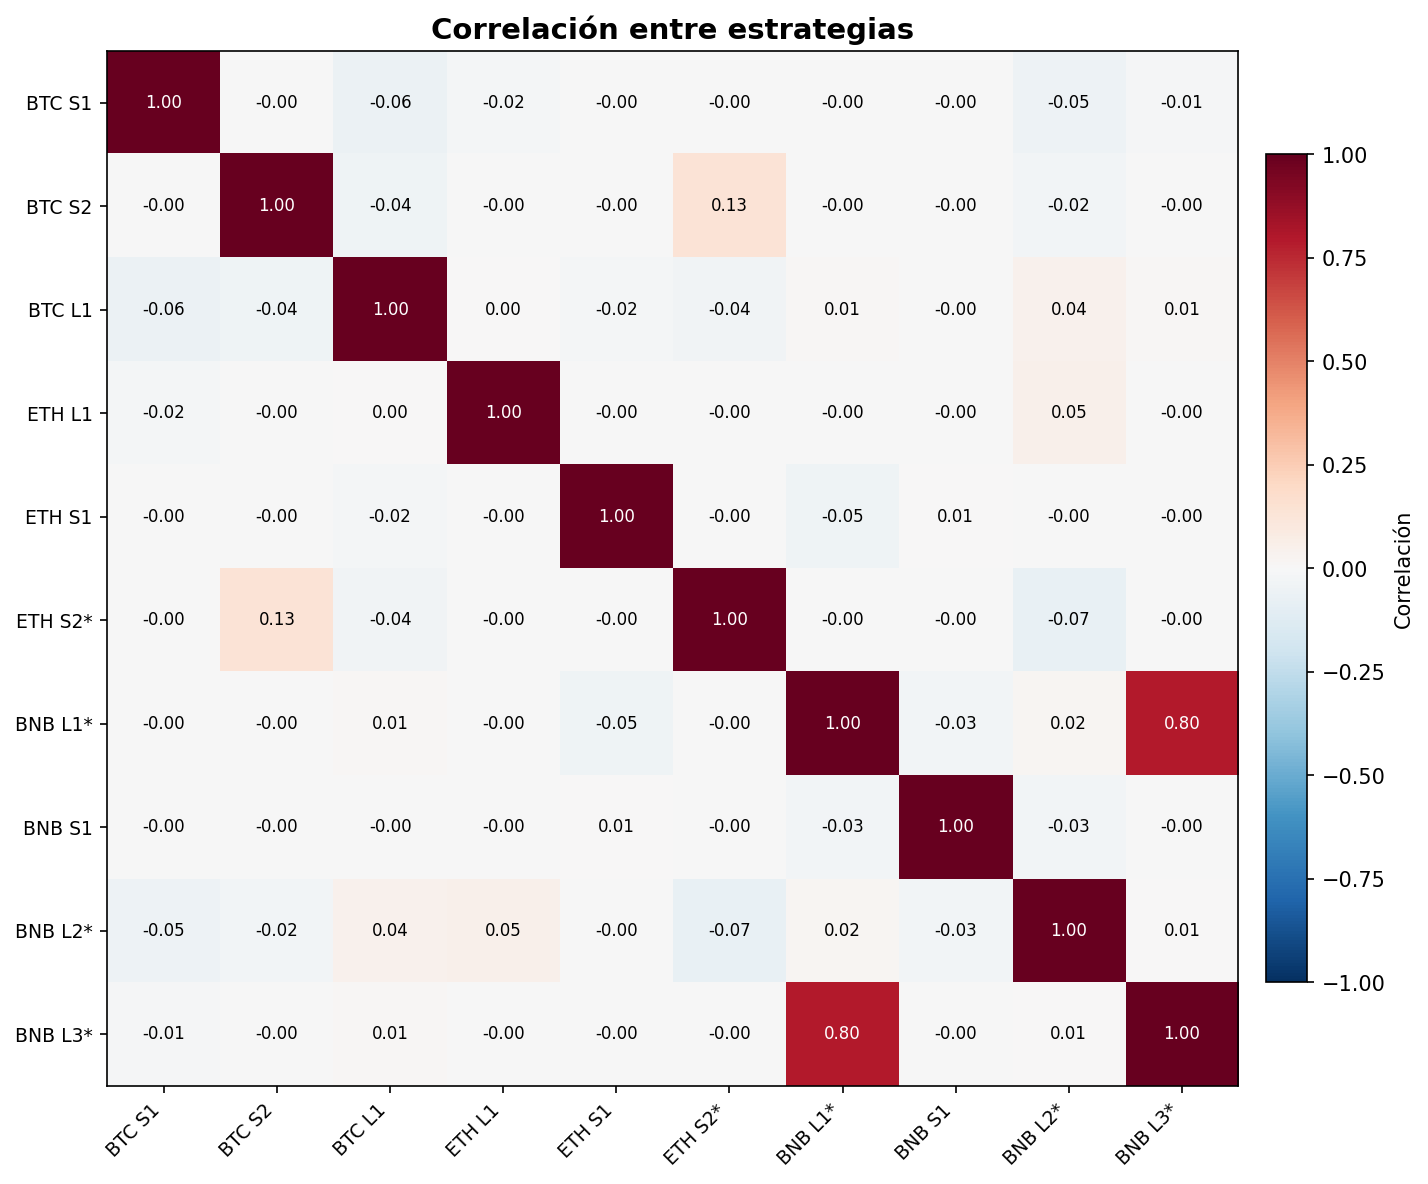
\includegraphics[width=0.75\textwidth]{figures/fig3_correlation.png}
\caption{Correlación entre las 10 estrategias del portafolio. La correlación promedio
es 0,014. La única excepción (0,80) son dos estrategias LONG de BNB.}
\label{fig:correlation}
\end{figure}

\subsection{Estabilidad walk-forward}

Para evaluar si los resultados se sostienen en el tiempo (y no solo en el período
OTS), se realizó una validación walk-forward: se aplicaron las estrategias sobre
10 ventanas temporales consecutivas de 2 meses cada una
(Tabla~\ref{tab:walkforward}).

\begin{table}[H]
\centering
\caption{Validación walk-forward por activo (10 ventanas consecutivas, con filtro
de régimen).}
\label{tab:walkforward}
\begin{tabular}{lcccc}
\toprule
\textbf{Activo} & \textbf{Ventanas +} & \textbf{Retorno acumulado} & \textbf{B\&H acumulado} & \textbf{Peor ventana} \\
\midrule
BTC & 9/10 (90\%) & +251\% & +188\% & $-$5,0\% \\
ETH & 9/10 (90\%) & +92,5\% & +52,9\% & $-$4,2\% \\
BNB & 8/10 (80\%) & +59,6\% & +270\% & $-$6,1\% \\
\bottomrule
\end{tabular}
\end{table}

BTC y ETH superan al buy-and-hold tanto en retorno como en consistencia. BNB logra
retornos inferiores al subyacente pero con un perfil de riesgo controlado: la peor
ventana individual es $-$6,1\% frente a caídas superiores al 30\% en el buy-and-hold.
La consistencia de 80--90\% de ventanas positivas sugiere que las estrategias capturan
patrones que persisten en el tiempo.

% ============================================================================
% 8. DISCUSIÓN
% ============================================================================
\section{Discusión}
\label{sec:discussion}

\subsection{El rol de la diversificación}

Los resultados confirman la hipótesis central del trabajo: sí es posible construir
un portafolio de patrones decorrelacionados con esperanza matemática positiva.
Las 10 estrategias tienen individualmente profit factor mayor a 1 (ganan más de
lo que pierden) y la correlación promedio entre ellas es de apenas 0,014. El efecto
es dramático: mientras las estrategias individuales tienen drawdowns de hasta
$-$23,6\%, el portafolio combinado no supera $-$3,5\%.

Esto es consistente con la teoría clásica de portafolios: cuando los activos (en este
caso, las curvas de equity de distintas estrategias) tienen correlación cercana a cero,
el riesgo del conjunto se reduce sin sacrificar proporcionalmente el retorno.

En este contexto, MAP-Elites cumple un rol que va más allá de la exploración
evolutiva: al forzar la diversidad comportamental, produce los ingredientes necesarios
para construir portafolios robustos. Una búsqueda que convergiera a una sola
``mejor'' estrategia no permitiría esta construcción.

\subsection{Interpretabilidad}

Una ventaja significativa de la Evolución Gramatical frente a enfoques de caja negra
(redes neuronales, reinforcement learning) es que las estrategias descubiertas son
\textit{legibles}. Cada regla puede expresarse como una combinación de condiciones
sobre indicadores técnicos conocidos, lo que permite:
\begin{itemize}
\item Verificar que la lógica tiene sentido económico (no es un artefacto numérico).
\item Comunicar la estrategia a otros investigadores o profesionales.
\item Diagnosticar fallos cuando las condiciones de mercado cambian.
\end{itemize}

Las estrategias descubiertas emplean combinaciones no triviales de indicadores ---por
ejemplo, combinar un filtro de sobreventa (RSI) con uno de expansión de volatilidad
(ancho de Bollinger) y uno de volumen--- que difícilmente un operador humano diseñaría
manualmente, pero que resultan interpretables una vez descubiertas.

\subsection{El ajuste fino funciona distinto según el activo}

Un resultado que no esperábamos: el ajuste fino de parámetros (CMA-ES) mejora las
estrategias de ETH y BNB pero empeora las de BTC. Una explicación posible es que BTC,
al ser el activo más líquido y más operado, deja menos margen: los parámetros que
encontró la evolución ya son casi los mejores posibles, y cualquier cambio los
empeora. En cambio, ETH y BNB tienen mercados menos eficientes donde sí hay espacio
para mejorar los parámetros. Esto sugiere que la decisión de aplicar o no este ajuste
debería depender del activo.

\subsection{Limitaciones}

\begin{enumerate}
\item \textbf{Indicadores técnicos estándar}: la gramática utiliza osciladores y ratios
  normalizados basados en precio y volumen. Datos alternativos (order flow,
  liquidaciones, métricas on-chain) podrían proveer señales complementarias.

\item \textbf{Una sola resolución temporal}: 15 minutos. Resoluciones mayores (1h, 4h,
  diaria) podrían capturar patrones de naturaleza diferente.

\item \textbf{Período de evaluación específico}: junio--noviembre 2025 fue un mercado
  predominantemente bajista. La validez de los resultados en otros entornos de mercado
  requiere investigación adicional.

\item \textbf{Costos simplificados}: se modelaron comisiones y slippage fijos; el
  impacto de mercado real podría diferir para volúmenes grandes.
\end{enumerate}

% ============================================================================
% 9. CONCLUSIONES Y TRABAJO FUTURO
% ============================================================================
\section{Conclusiones y Trabajo Futuro}
\label{sec:conclusions}

\subsection{Conclusiones}

Este trabajo presentó un framework de descubrimiento automatizado de estrategias
cuantitativas que combina Evolución Gramatical, MAP-Elites, optimización local con
CMA-ES y validación estadística rigurosa. Los resultados principales son:

\begin{enumerate}
\item El algoritmo evolutivo demostró ser capaz de explorar un espacio de
  $\sim$$10^8$ reglas posibles evaluando menos del 0,03\% del total, pero
  concentrándose en las zonas prometedoras. Descubrió estrategias interpretables
  que un humano difícilmente diseñaría a mano.

\item El mecanismo de diversidad (MAP-Elites) mantuvo estrategias variadas ---unas
  para mercado alcista, otras para bajista; unas simples, otras complejas--- y esa
  diversidad resultó ser el ingrediente clave para armar portafolios robustos.

\item La optimización en dos fases (evolución para estructura, CMA-ES para
  parámetros) mejoró las estrategias de ETH y BNB pero no las de BTC, lo que
  sugiere que en mercados más líquidos queda menos margen para ajustar.

\item El pipeline de validación (CPCV + PBO + permutación) filtró eficazmente las
  estrategias sobreajustadas: de 166 candidatas en BTC, 87 superaron los tres
  criterios simultáneamente.

\item El framework generalizó a tres activos con microestructuras diferentes. La
  validación walk-forward mostró consistencia del 80--90\% de ventanas positivas
  en BTC, ETH y BNB. El portafolio multi-activo de 10 estrategias obtuvo un
  CAGR de 36,5\%, drawdown máximo de $-$3,5\%, Sharpe de 3,4 y una correlación
  promedio entre estrategias de apenas 0,014 ---confirmando que es posible construir
  un portafolio de patrones decorrelacionados con esperanza matemática positiva.
\end{enumerate}

\subsection{Trabajo futuro}

Varias extensiones podrían ampliar el alcance de los resultados:

\begin{itemize}
\item \textbf{Aprendizaje por refuerzo}: usar las estrategias descubiertas como
  política inicial para un agente de RL, combinando la interpretabilidad de GE con
  la capacidad adaptativa del aprendizaje por refuerzo.

\item \textbf{Señales multi-resolución}: combinar indicadores calculados sobre velas
  de 15 minutos, 1 hora y 4 horas para capturar patrones jerárquicos. La gramática
  actual soporta esta extensión, pero los experimentos presentados se limitan a la
  resolución de 15 minutos.

\item \textbf{Datos alternativos}: incorporar métricas de flujo de órdenes, tasas de
  financiamiento e indicadores on-chain como terminales adicionales en la gramática.

\item \textbf{Position sizing adaptativo}: evolucionar reglas de tamaño de posición
  como parte del genoma, utilizando señales de régimen de volatilidad (por ejemplo,
  modelos HMM) para modular la exposición.

\item \textbf{Co-evolución competitiva}: evolucionar poblaciones de estrategias que
  compiten entre sí, simulando la dinámica de un mercado con múltiples participantes
  informados.
\end{itemize}

\end{document}
